% Birth-death process.
\documentclass[11pt,tikz,border=2pt]{standalone}
\usepackage{tikz}
\usetikzlibrary{arrows}
\begin{document}
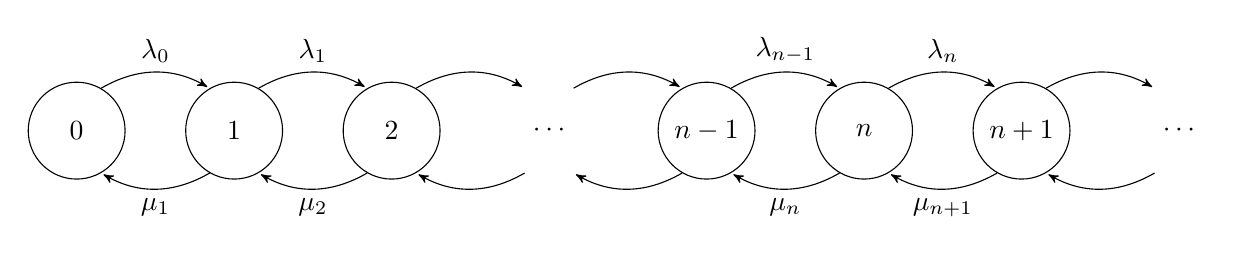
\begin{tikzpicture}[->,>=stealth',shorten >=1pt,auto,node distance=2cm,
		main node/.style={circle,draw,minimum size=35pt},
		invis node/.style={circle,minimum size=35pt}]
	\node[main node] (0) {0};
	\node[main node] (1) [right of=0] {$1$};
	\node[main node] (2) [right of=1] {$2$};
	\node[invis node] (3) [right of=2] {$\cdots$};
	\node[main node] (4) [right of=3] {$n-1$};
	\node[main node] (5) [right of=4] {$n$};
	\node[main node] (6) [right of=5] {$n+1$};
	\node[invis node] (7) [right of=6] {$\cdots$};
	\path[]
		(0.60) edge [bend left] node {$\lambda_0$} (1.120)
		(1.60) edge [bend left] node {$\lambda_1$} (2.120)
		(2.60) edge [bend left] node {} (3.120)
		(3.60) edge [bend left] node {} (4.120)
		(4.60) edge [bend left] node {$\lambda_{n-1}$} (5.120)
		(5.60) edge [bend left] node {$\lambda_{n}$} (6.120)
		(6.60) edge [bend left] node {} (7.120);
	\path[]
		(7.240) edge [bend left] node {} (6.300)
		(6.240) edge [bend left] node {$\mu_{n+1}$} (5.300)
		(5.240) edge [bend left] node {$\mu_{n}$} (4.300)
		(4.240) edge [bend left] node {} (3.300)
		(3.240) edge [bend left] node {} (2.300)
		(2.240) edge [bend left] node {$\mu_2$} (1.300)
		(1.240) edge [bend left] node {$\mu_1$} (0.300);
\end{tikzpicture}
\end{document}
